\documentclass[a4paper]{article}
\usepackage[utf8]{inputenc}
\usepackage[spanish, es-tabla]{babel}

\usepackage{amsmath}
\usepackage{amsfonts}
\usepackage{amssymb}

\usepackage{float}
\usepackage{graphicx}
\graphicspath{ {./Imagenes/} }

\usepackage{multirow}
\setlength{\doublerulesep}{\arrayrulewidth}

\usepackage[american]{circuitikz}

\usepackage{fancyhdr}

\usepackage{units} 

\pagestyle{fancy}
\fancyhf{}
\lhead{22.02 Electrotecnia I}
\rhead{Mechoulam, Mestanza, Lambertucci, Pouthier, Londero}
\rfoot{Página \thepage}



\begin{document}

%%%%%%%%%%%%%%%%%%%%%%%%%%%%%%%%%%%%%%%%%%%%%%%%%%%%%%%%%%%%%%%%%%%%%%%%% 
%								CARATULA								%
%%%%%%%%%%%%%%%%%%%%%%%%%%%%%%%%%%%%%%%%%%%%%%%%%%%%%%%%%%%%%%%%%%%%%%%%% 

\begin{titlepage}
\newcommand{\HRule}{\rule{\linewidth}{0.5mm}}
\center
\mbox{\textsc{\LARGE \bfseries {Instituto Tecnológico de Buenos Aires}}}\\[1.5cm]
\textsc{\Large 22.02 Electrotecnia I}\\[0.5cm]


\HRule \\[0.6cm]
{ \Huge \bfseries Trabajo práctico N$^{\circ}$3}\\[0.4cm] 
\HRule \\[1.5cm]


{\large

\emph{Grupo 5}\\
\vspace{3px}

\begin{tabular}{lr} 	
\textsc{Mechoulam}, Alan  &  58438\\
\textsc{Lambertucci}, Guido Enrique  & 58009 \\
\textsc{Pouthier}, Florian  & 61337 \\
\textsc{Mestanza}, Nicolás  & 57521 \\
\textsc{Londero Bonaparte}, Tomás Guillermo  & 58150 \\
\end{tabular}

\vspace{20px}

\emph{Profesores}\\
\vspace{3px}
\textsc{Muñoz}, Claudio Marcelo\\ 	
\textsc{Ayub}, Gustavo\\ 	

\vspace{100px}

\begin{tabular}{ll}

Presentado: & 17/05/19\\

\end{tabular}

}

\vfill

\end{titlepage}


%%%%%%%%%%%%%%%%%%%%%%%%%%%%%%%%%%%%%%%%%%%%%%%%%%%%%%%%%%%%%%%%%%%%%%%%% 
%								INFORME									%
%%%%%%%%%%%%%%%%%%%%%%%%%%%%%%%%%%%%%%%%%%%%%%%%%%%%%%%%%%%%%%%%%%%%%%%%%

\section*{Introducción}

En el trabajo realizado se observó el funcionamiento de un transformador. Se realizaron análisis en del circuito modelando sistemas en corto, en vacío y con carga. 


\section*{Desarrollo de la experiencia}

\section[I]{\underline{Primera parte}}

Para empezar se dispuso el circuito de la forma mostrada en la figura (\ref{fig:1a}). Luego, se colocó un voltímetro en los distintos bornes de las inductacias, para poder, de esta forma, determinar de que manera serían homólogos, sabiendo que se daría dicha condición cuando la diferencia de tensión sea próxima a cero.

\begin{figure}[H]
	\centering
	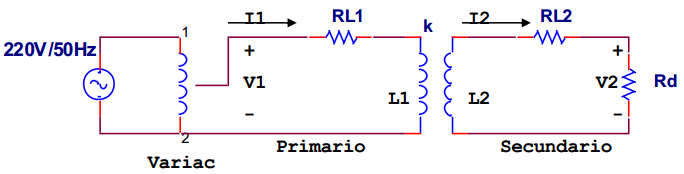
\includegraphics[width=0.8\textwidth]{Circuito-1.PNG}
	\caption{Circuito empleado.}
	\label{fig:1a}
\end{figure}

Así queda determinado el sentido de la inductancia mutua, conectando el voltimetro de forma en la que se muestra en la figura (\ref{cir:1a}).

\begin{figure}[H]
\begin{center}
\begin{circuitikz}
	\draw
		
	(1,0) node[transformer] (T) {}
	node[ocirc] (A) at ([xshift=-1cm]T.A1) {}
	node[ocirc] (B) at ([xshift=-1cm]T.A2) {}
	node[ocirc] (C) at ([xshift=1cm]T.B1) {}
	node[ocirc] (D) at ([xshift=1cm]T.B2) {}
	node[circ] (E) at ([xshift=0.4cm,yshift=-5pt]T.A1) {}
	node[circ] (F) at ([xshift=-0.4cm,yshift=-5pt]T.B1) {}
	(T.A1) to	[-o] (A)
	(T.A2) to	[-o] (B) 
	(T.B1) to	[-o] (C)
	(T.B2) to	[-o] (D)
	(T.west) node{$L_1$}
	(T.east) node{$L_2$}

	(0,0.5)	to	node[draw,circle,fill=white] {V} (2,0.5)
	(0,0)	to	(0,0.5)
	(2,0)	to	(2,0.5)

	;\end{circuitikz}
\end{center}
\caption{Determinación del sentido de M.}
\label{cir:1a}
\end{figure}

Una vez hecho lo mencionado anteriormente, se prosigue conectando las herramientas necesarias en el circuito para realizar las mediciones adecuadas.

\begin{figure}[H]
\begin{center}
\begin{circuitikz}
	\draw
		
	(-1, -1.1) 		to [vL] (-1,-2.1)
	(-1.5, -1.1) 	to [short, *-] (-1, -1.1)
	(-1.5, -2.1) 	to [short, *-] (-1, -2.1)
					to (0,-2.1)
	(0,0)	to (0,-1.7)
			to (-0.6,-1.7)
	(0,0) 	to node[draw,circle,fill=white] {A} (1.5, 0)
			to (3.5,0) to [R, l=$R_{L_{1}}$] (5.5,0)
			
	(2.5,0) to node[draw,circle,fill=white] {V} (2.5, -2.1)
	
	(0,-2.1) to (5,-2.1) to (5.5,-2.1)	

	(6.5,0) node[transformer core]{}
	(7.5,0) to [R, l=$R_{L_{2}}$] (9.5,0) to (10,0)
	(7.5,-2.1) to (10,-2.1)
	(10,0) to [vR, l_ = $R_d$] (10,-2.1)

	;\end{circuitikz}
\end{center}
\caption{Circuito analizado.}
\label{cir:1b}
\end{figure}

Luego se determinaron mediante el uso de un ohmetro las resistencias internas de cada bobina siendo $ R_1 = 23 \ \Omega $ y $ R_2 = 21,8 \ \Omega $ la del primario y del secundario respectivamente.

Por último se procedió a realizar las mediciones adecuadas y se calcularon los valores de auto inductancia, el factor de acoplamiento y el valor de mutua inductancia. Dichos resultados y cálculos se encuentran en la tabla (\ref{tabla:1a}). Cabe aclarar que algunos valores, tales como el coeficiente de acoplamiento y las auto inductancias, no pudieron ser calculados en aquellos análisis en vacío. 


\begin{table}[H]
\centering
\begin{tabular}{|c|c|c|c|c|c|c|c|c|c|}
\hline
\textbf{Caso}                                                             & \textbf{\begin{tabular}[c]{@{}c@{}}$V_1$\\ {[}V{]}\end{tabular}} & \textbf{\begin{tabular}[c]{@{}c@{}}$I_1$\\ {[}A{]}\end{tabular}} & \textbf{\begin{tabular}[c]{@{}c@{}}$V_2$\\ {[}V{]}\end{tabular}} & \textbf{\begin{tabular}[c]{@{}c@{}}$I_2$\\ {[}A{]}\end{tabular}} & \textbf{\begin{tabular}[c]{@{}c@{}}$R_D$\\ $\Omega$\end{tabular}} & \textbf{\begin{tabular}[c]{@{}c@{}}M\\ {[}H{]}\end{tabular}} & \textbf{k} & \textbf{\begin{tabular}[c]{@{}c@{}}$L_1$\\ {[}H{]}\end{tabular}} & \textbf{\begin{tabular}[c]{@{}c@{}}$L_2$\\ {[}H{]}\end{tabular}} \\ \hline
\textbf{Hierro Sólido}                                                    & 93,4                                                             & 0,3                                                              & 14,6                                                             & 0,06                                                             & 200                                                               & 0,15                                                         & 0,28       & 0,99                                                             & 0,32                                                             \\ \hline
\textbf{Laminado}                                                         & 93,4                                                             & 0,45                                                             & 23,22                                                            & 0,1                                                              & 200                                                               & 0,26                                                         & 0,33       & 0,66                                                             & 0,93                                                             \\ \hline
\textbf{\begin{tabular}[c]{@{}c@{}}Laminado\\ ($I_2 = 0$)\end{tabular}}   & 93,4                                                             & 0,4                                                              & 33,22                                                            & 0                                                                & 0                                                                 & -                                                            & -          & -                                                                & -                                                                \\ \hline
\textbf{\begin{tabular}[c]{@{}c@{}}Sin núcleo\\ ($I_2 = 0$)\end{tabular}} & 93,4                                                             & 0,8                                                              & 8,3                                                              & 0                                                                & 0                                                                 & -                                                            & -          & -                                                                & -                                                                \\ \hline
\end{tabular}
\caption{Mediciones realizadas en la primer experiencia.}
\label{tabla:1a}
\end{table}


\section{\underline{Segunda parte}}

En esta parte, se hace un análisis práctico de un transformador monofásico. El dicho es construido de la misma manera que en la primera parte, con dos bobinas y un núcleo de hierro.

El objetivo es hallar los parámetros físicos de este transformador con diferentes ensayos sucesivos.

Con un transformador de este tipo, no es posible estimar el rendimiento o regulación, porque ...

\subsection{Ensayo en vacío}

Para este primer ensayo, se procede al armado del siguiente circuito:

\begin{figure}[H]
\begin{circuitikz}
\draw
	(-1, -1.1) 		to [vL] (-1,-2.1)
	(-1.5, -1.1) 	to [short, *-] (-1, -1.1)
	(-1.5, -2.1) 	to [short, *-] (-1, -2.1)
					to (0,-2.1)
	(0,0)	to (0,-1.7)
			to (-0.6,-1.7)
	(0,0) 	to node[draw,circle,fill=white] {A} (1.5, 0)
			to node[draw,circle,fill=white] {W} (3.5, 0)
			to [short, -*] (5, 0) to (5.5,0)
	(0.7,0.7) node[]{$I_{10}$}
	(2.5,0.7) node[]{$P_{10}$}
	(2.5,-0.4) to (2.5,-2.1)
	(4,0) to node[draw,circle,fill=white] {V} (4, -2.1)
	(4.5,-0.5) node[]{$U_{10}$}
	(0,-2.1) to [short, -*] (5,-2.1) to (5.5,-2.1)
	(6.5,0) node[transformer core]{}
	(8,0) to (7,0) to [short, -*] (9.5,0)
	(8,-2.1) to (7,-2.1) to [short, -*] (9.5,-2.1)
	(8.5,0) to node[draw,circle,fill=white] {V} (8.5, -2.1)
	(9,-0.5) node[]{$U_{20}$};
\end{circuitikz}
\caption{Circuito analizado durante la segunda instancia.}
\end{figure}

Aplicando una tensión nominal cercana de 100 V, el vatímetro indicará las pérdidas en el hierro nominales. A continuación, se representa un forma de tabla, los calores medidos y calculados de dicho anlisis

\begin{table}[H]
\centering
\begin{tabular}{|c|c|c|c|c|c|c|c|c|c|c|}
\hline
\textbf{Parámetro} & \textbf{\begin{tabular}[c]{@{}c@{}}$U_{10}$\\ {[}V{]}\end{tabular}} & \textbf{\begin{tabular}[c]{@{}c@{}}$U_{20}$\\ {[}V{]}\end{tabular}} & \textbf{\begin{tabular}[c]{@{}c@{}}$I_{10}$\\ {[}A{]}\end{tabular}} & \textbf{\begin{tabular}[c]{@{}c@{}}$P_{10}$\\ {[}W{]}\end{tabular}} & \textbf{$cos \ \phi$} & \textbf{\begin{tabular}[c]{@{}c@{}}$I_{m}$\\ {[}A{]}\end{tabular}} & \textbf{\begin{tabular}[c]{@{}c@{}}$I_{p}$\\ {[}A{]}\end{tabular}} & \textbf{\begin{tabular}[c]{@{}c@{}}$R_{p}$\\ {[}$\Omega${]}\end{tabular}} & \textbf{\begin{tabular}[c]{@{}c@{}}$X_{m}$\\ {[}$\Omega${]}\end{tabular}} & \textbf{\begin{tabular}[c]{@{}c@{}}$M$\\ {[}H{]}\end{tabular}} \\ \hline
\textbf{Valor}     & 93,1                                                                & 35,2                                                                & 0,375                                                               & 6,75                                                                & 0,193                 & 0,368                                                              & 0,073                                                              & 1284,09                                                                   & 253,041                                                                   & 0,378                                                          \\ \hline
\end{tabular}
\caption {Ensayo a circuito abierto.}
\end{table}



\subsection{Ensayo en cortocircuito}
Se Buscó determinar las pérdidas debidas al devanado de cobre del transformador. Para esto, se conectó un vatímetro en el primario y se concretó que la medición realizada con este son las pérdidas, ya que la única resistencia del circuito es la del cobre. A continuación se detallan los resultados obtenidos.

\begin{table}[H]
\centering
\begin{tabular}{|c|c|c|c|c|c|c|c|}
\hline
\textbf{Parámetro} & \textbf{\begin{tabular}[c]{@{}c@{}}$U_{1CC}$\\ {[}V{]}\end{tabular}} & \textbf{\begin{tabular}[c]{@{}c@{}}$I_{1CC}$\\ {[}A{]}\end{tabular}} & \textbf{\begin{tabular}[c]{@{}c@{}}$I_{2CC}$\\ {[}A{]}\end{tabular}} & \textbf{\begin{tabular}[c]{@{}c@{}}$P_{1CC}$\\ {[}W{]}\end{tabular}} & \textbf{$cos \ \phi$} & \textbf{\begin{tabular}[c]{@{}c@{}}$R_{1} = R_{21}$\\ {[}$\Omega${]}\end{tabular}} & \textbf{\begin{tabular}[c]{@{}c@{}}$X_{1} = X_{21}$\\ {[}$\Omega${]}\end{tabular}} \\ \hline
\textbf{Valor}     & 91,4                                                                 & 0,448                                                                & 0,16                                                                 & 8,625                                                                & 0,211                 & 336,9                                                                              & 1561,79                                                                            \\ \hline
\end{tabular}
\caption {Ensayo a corto circuito}
\centering
\end{table}
\subsection{Modelo resultante del transformador}



\end{document}
